\section{Introduction}
The goal of this project was to create a more modernised version of Robotron: 2084, the classic arcade game from the 80s. In order to make it a more modern version I will make a few additions, including improving the game itself and increase the competition aspect of it. I also needed to modernise the codebase itself, and couldnt build off the existing code written in the 80s.

As i was unable to access the code from the original game, nor find a viable method to emulate the code on my machine, i was forced to take my research from websites, videos and images, and whilst this isnt ideal, i was still able to gain a vast amount of information and replicate the game how i wanted to.

Whilst there is no specific target audience for the project, it could be played and enjoyed by anyone, ranging from my classmates to the people who played and enjoyed the original game from the 80s. Thanks to the wide range of possible users, there is a large market i can test this app with.

\section{About the game}

Robotron 2084 is a classic, top down, arcade game from the 80's, in which, a player (who is a mutant genetic super hero) attempts to save the last human family from swarms of killer robots. The game was a 2 stick shooter originally - this means 2 joysticks, one to move and one to shoot (this allows the 2 to occur individually and simultaneously). This was one of the first of its kind, and was largely considered a success. The game has a number of waves with varying number or robots, of different types, and varying numbers of humans.

In order to 'save' a human, they player simply has to touch them, this rescues the human and scores the player points. The more humans saved, the higher the points. The player, whilst a mutant, is still susceptible to damage - and whilst there is no 'health' the player can be killed rather easily. The robots simply have to touch the player (or the player accidentally collide with them) and the player 'dies'. You start the game with 3 lives and slowly progress through the waves - a new wave starts when all of the grunts (one of the robots, see table below) are killed, or when the player dies. 
There are also various transition screens, including a boot screen, a testing screen and end screens. Along with these come a live counter, a score counter and flashing borders. The game is fast passed and bright, and graphically complex, with lots of colours and intense action. Making a game like this play as smoothly as they did at the time was truly an accomplishment.
The game even had sound! whilst it was only mono aural (no stereo) - this was still impressive, considering it was a game running on a 1MHz processor. They were able to develop this in a 2 man team over a period of 6 months. It was itself heavily influenced by a number of other games, including 'Berzerk' - a shooting game which players traverse a maze and shoot at enemies. However, this was a single stick shooter (with a button to fire) rather than a dual stick shooter.
The game had sequels but none were as successful as the original, and were never received as well. One even attempted a multiplayer system, where one would shoot and another would move, but this was not widely seen as a positive update.

\section{More Modern 2D games}
In order to bring this game into the 21st century, it will need more modernised features. For one, almost everyone plays games on computers, and as such, will need a 'dual stick' implementation. Almost every modern game uses WASD to move and arrows to shoot, but IJKL is also used to shoot. Other approaches to avoid seeming like a single stick shooter are using the mouse to control movement or shooting, or even ESDX and IJKM as move and shoot (this was the original set up for Robotron 2084 on apple products. 

\section{Robotron's Design}
I mostly used video for my research into robotrons design - this felt like the best way due to how fast the game changes, with fast animations and colour changes, something that cannot be captured easily in photo screenshots. I also relied on websites, also linked, for more technical information and this is where i was also able to learn lots of the history behind the game.


\begin{itemize}
    \item \url{https://www.youtube.com/watch?v=ccltMtkFBSI} - This video - impressive in itelf for the gameplay, gave me more of an insight into the feel of the past paced nature of the game, and whilst the quality isnt perfect, it gives some idea of the general layout of the screen and game
    
    \item \url{https://www.youtube.com/watch?v=aOVA2Axxfdk} - This video was much higher quality screen capture of the game, this is what allowed me to see animation and character design as well as have a very good understanding of what layouts looked like, and the general interface.
    
    \item \url{https://arcadeblogger.com/2020/06/27/the-development-of-robotron/} This was possibly my most used resource. Having insight into the development and original views of the game was very important, and this website alone would probably have been enough to implement it. 
\end{itemize}

Whilst i didn't want to build a carbon copy of the original, i did endeavour to create something as similar as i could without loosing too much of the fast paced nature of the game.


\section{Robotron Step by Step}
Robotron starts up with a pattern of random pixels, followed by a screen indicating that tests were successful (or, as it may be, unsuccessful), before finally transitioning to the start screen. This screen has the words Robotron, along with credits to the developer. It is very bright, and flashing. The game also has a high score board displaying at the end of every run (and i believe it would also display at times when the machine was not in game). When starting the game, it would show a level transition screen (bright rectangles would display from the centre of the screen moving out). A wave would then start. This would begin by displaying all character, but not allowing movement of enemies for a few moments (this is probably a design choice, a brief moment for the player to plan their first few movements, and analyse where they should head). The levels would then loop like this, with a transition showing between each.

To illustrate the game layout better, i have included a finite state machine of how the game would work, it can be found below in \ref{fig:Robotron_FSM}.

\begin{figure}[ht!]
  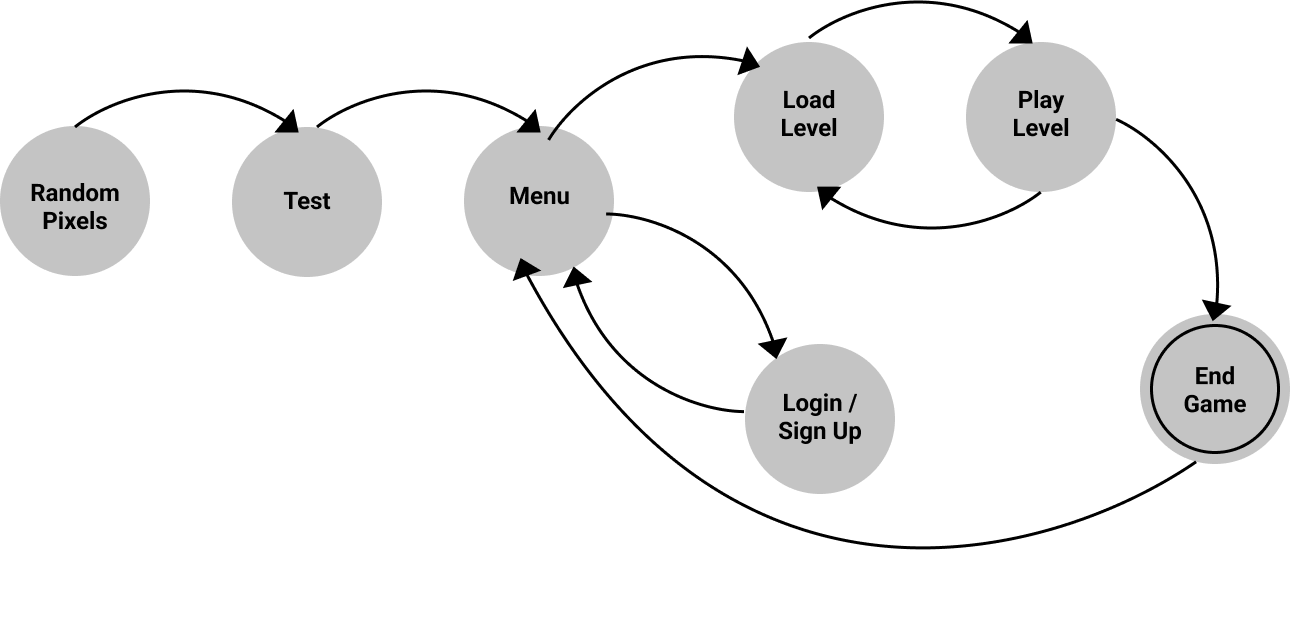
\includegraphics[width=0.8\linewidth]{Figures/FSM_robotrom.png}
  \centering
  \caption{The FSM which shows a very basic overview of how robotron 2084 works}
  \label{fig:Robotron_FSM}
\end{figure}


\section{Enemy Specific Behaviour}
One problem with not having access to the original code is the inability to tell what algorithm was used to cause the grunt enemy to 'flock' to the player (the only enemy I will implement which is actively seeking to get to the player) there are a few ways i could have done this, almost all of them much more simple than the method I would end up on.

A very basic approach to creating something like this is to simply move in the direction of the player, at a speed of x pixels per blit. This would have lead to some issues though. The main one being crowding. This would allow lots of grunts to 'stack', making it easier to kill them (a stream of bullets into this stack, and they are all destroyed). As such, this was rejected. I considered adding a random element to this (like having them move at a random speed, or adding some random direction) - but this would risk the grunts becoming jittery.

The solution is to use an algorithm called 'boids'. It is known as an artificial life program, and is meant to mimic the flocking of birds (boids = bird-oid object). It works by applying individual rules to each boid (each item in the flock) which results in a hive mind sort of intelligence. It is made up of 3 basic rules, plus 1 more to allow the group to move towards the goal (in this case the player).

\subsection{Rule 1 - move to centre mass}
First, calculate the centre of mass, for the boids in view. Essentially, sum all x and y co ordinate values and divide by the number of boids, for the co ordinates of the centre (c) $(\frac{\Sigma x}{n_{boids}},\frac{\Sigma y}{n_{boids}})$. Then, we want to move the boid 1\% of the way towards this centre, so our actual movement vector is given by $\frac{c - P_{boid}}{100}$ (where $P_{boid}$ is the position of the currently calculated boid), we need to subtract $P_{boid}$ as we want to move 1\% of the distance from the current position, not from the position $(0,0)$.
    
\subsection{Rule 2 - Avoid collisions with other boids}
This one is much more simple. For this, we simply want to move away from the other boids. To do that, just add the magnitudes of the difference between the 2 current positions to get a new position. 

\subsection{Rule 3 - Match velocities of the other boids}
This is also somewhat complex but works like Rule 1. We want to have the boids attempt to match the velocities of the boids around it. This could be done with some similar maths. First, sum all the velocities (V) $(\frac{\Sigma V_x}{n_{boids}},\frac{\Sigma V_y}{n_{boids}})$, much like with Rule 1, we dont want to match this velocty perfectly. Instead, add about a twentieth of the calculated value, which can be performed with $\frac{V - V_{boid}}{20}$

\subsection{Rule 4 - Move towards the player}
This rule is easy. Find the distance to the player, and move about a 5th of the way there.

\subsection{Notes on boids}
I did not create the boids flocking algorithm. It was created by Craig Reynolds, \url{http://www.red3d.com/cwr/boids/} is where i pulled most of my information from. This is a tweaked version from the original, with altered values that i set to perform more how i wanted (eg, to emulate a hoard of robots over flocking birds) and with the added rule of moving towards a player. 

\section{Python Library selection}
I had to select python libraries to handle 2 large sections of my code, these were the web framework and the gui framework. These both are hugely popular areas of python development, and there are a multitude of frameworks which i would have used, but there were 2 major contenders for each.

\subsection{Web Framework Library}
This was a relatively simple choice, flask or django. I had already decided that this would be a relatively simple website with a need for a larger focus to the API, and less need for web content. As such, django makes less sense, and flask is much faster, so this was quite an easy solution to use. In the past I've also found flask easier to deploy and debug, certainly it was my preference of backend anyway - but it also made sense.

\subsection{GUI Library}
Python has a few possible libraries, but again, 2 main contenders. TkInter and PyGame. TkInter is built in, and i have used it in the past, but when I used it, I used it for fairly basic forms, and at most, a chess game. These were no fast paced, and I wasnt convinced it would handle the huge number of sprites and fast moving objects. As such, I decided to go with Pygame, which is much better suited to this.

\section{Game Code Architecture}
Selecting an architecture was important. It was clear from the get go that this project would heavily use OOP, as it made sense, not just for sprites in general but also for its ease of use with pygame. I could have had a very simple system with a game loop and processing in there. I eventually settled on a specific design, and that was MVC (Model-View-Controller) as an architecture for the game.  This divides the logic into 3 components, 1, the model, which handles all the data, and is esentially the 'backend' of the game; 2, the view, this is the part the user sees, and is fed from the model, and finally, the controller, which is how the user interacts with the machine, and this feeds the model. 

For example, whilst it may have been possible to have it so that whenever a WASD key is pressed, the view is instantly moved to show the updated position - MVC dictates that you first update the model, and then on the next blit this update gets drawn up. This may seem somewhat counter intuative, but means each component can be swapped out much easier, leading to an incredibly modular design. This makes it much easier to develop, improve and test.

The system will also use a state machine (implemented with a stack) to control what is currently shown on screen as each state has its own meaning and definitions of what is needed on screen. Again, this allows for a much more modular system, as individual functions can be called once the current state is identified. It will also have an event system - such that it is a largely data driven system, where data is processed on the fly as it is received.

\section{Objectives}
\begin{easylist}[articletoc]
@ Game Objectives
@@ Main (hero) character objectives
@@@ Character can be displayed
@@@ Character can move in all 8 directions
@@@ Character faces in correct direction
@@@ Characters movement is animated
@@@ Character is bounded to window
@@@ Character can shoot in 8 directions
@@@ Player is invincible on load of level
@@ Enemy character objectives (for each enemy type - Electrodes, Grunts and Hunks)
@@@ Enemies can be displayed
@@@ Enemies can move
@@@ Enemy faces correct direction
@@@ Enemies movement is animated
@@@ Enemy are bounded to window
@@@ Enemy kills player when touching
@@@ Specific enemy functionality
@@@@ Electrodes are randomly spread around the page
@@@@ Grunts flock around player
@@@@ Hunks slow down when shot
@@ Menu objectives
@@@ Logo is shown and animated
@@@ Display static text
@@@ Display animated text
@@@ Display and allow input for options
@@@ Allow for login and sign up
@@ Extras objectives (additional features) 
@@@ Flashing border
@@@ Random colour load screen
@@@ "All tests" screen
@@@ Inter---level animation
@@@ Sounds
@@@@ For shooting
@@@@ For start up
@@@@ For level change

@ Website Objectives
@@ Displays high score board of top 10 players
@@ Website animated and looks like the high score board on original game
@@ Have an error page, informs user something went wrong
@@ API Goals (a route to...)
@@@ Return top scores
@@@ Allow for sign up
@@@ Allow for log in
@@@ Generate tokens for login
@@@ Upload scores and validate with token
\end{easylist}